%%%%%%%%%%%%%%%%%%%%%%%%%%%%%%%%%%%%%%%%%
% Beamer Presentation
% LaTeX Template
% Version 1.0 (10/11/12)
%
% This template has been downloaded from:
% http://www.LaTeXTemplates.com
%
% License:
% CC BY-NC-SA 3.0 (http://creativecommons.org/licenses/by-nc-sa/3.0/)
%
%%%%%%%%%%%%%%%%%%%%%%%%%%%%%%%%%%%%%%%%%

%----------------------------------------------------------------------------------------
%	PACKAGES AND THEMES
%----------------------------------------------------------------------------------------

\documentclass[aspectratio = 1610, xcolor = dvipsnames]{beamer}
\usefonttheme{serif} % default family is serif


\usepackage{changepage}
\usepackage{verbatim}
\usepackage[english]{babel}
\usepackage[utf8]{inputenc}

\usepackage{subfigure} % Allows including images
\usepackage{wrapfig}
\usepackage{booktabs, multirow} % Allows the use of \toprule, \midrule and \bottomrule in tables
\usepackage[rounded, shadow]{beamerinnerthemerounded}
\usepackage{soul}



\usepackage[backend=biber,style=authortitle, sorting=none]{biblatex}
\bibliography{bibliography}

\usepackage{csquotes}



%\setbeamersize{text margin left=2mm,text margin right=2mm} 

% The Beamer class comes with a number of default slide themes
% which change the colors and layouts of slides. Below this is a list
% of all the themes, uncomment each in turn to see what they look like.

%\usetheme{default}
%\usetheme{AnnArbor}
%\usetheme{Antibes}
%\usetheme{Bergen}
%\usetheme{Berkeley}
\usetheme{Berlin}
%\usetheme{Boadilla}
%\usetheme{CambridgeUS}
%\usetheme{Copenhagen}
%\usetheme{Darmstadt}
%\usetheme{Dresden}
%\usetheme{Frankfurt}
%\usetheme{Goettingen}
%\usetheme{Hannover}
%\usetheme{Ilmenau}
%\usetheme{JuanLesPins}
%\usetheme{Luebeck}
%\usetheme{Madrid}
%\usetheme{Malmoe}
%\usetheme{Marburg}
%\usetheme{Montpellier}
%\usetheme{PaloAlto}
%\usetheme{Pittsburgh}
%\usetheme{Rochester}
%\usetheme{Singapore}
%\usetheme{Szeged}
%\usetheme{Warsaw}

% As well as themes, the Beamer class has a number of color themes
% for any slide theme. Uncomment each of these in turn to see how it
% changes the colors of your current slide theme.

%\usecolortheme{albatross}
%\usecolortheme{beaver}
%\usecolortheme{beetle}
%\usecolortheme{crane}
%\usecolortheme{dolphin}
%\usecolortheme{dove}
%\usecolortheme{fly}
\usecolortheme{lily}
%\usecolortheme{orchid}
%\usecolortheme{rose}
%\usecolortheme{seagull}
%\usecolortheme{seahorse}
%\usecolortheme{whale}
%\usecolortheme{wolverine}




\makeatletter
\setbeamertemplate{footline}
{
	\leavevmode%
	\hbox{%
		\begin{beamercolorbox}[wd=.333333\paperwidth,ht=2.25ex,dp=1ex,center]{author in head/foot}%
			\usebeamerfont{author in head/foot}Javier Mariño Villadamigo
		\end{beamercolorbox}%
		\begin{beamercolorbox}[wd=.333333\paperwidth,ht=2.25ex,dp=1ex,center]{title in head/foot}%
			\usebeamerfont{title in head/foot}Research Activities % at slide bottom
		\end{beamercolorbox}%
		\begin{beamercolorbox}[wd=.333333\paperwidth,ht=2.25ex,dp=1ex,right]{date in head/foot}%
			\usebeamerfont{date in head/foot}\insertshortdate{}\hspace*{2em}
			\insertframenumber{} / \inserttotalframenumber\hspace*{2ex} 
	\end{beamercolorbox}}%
	\vskip0pt%
}
\makeatother


\makeatletter
\@addtoreset{subfigure}{framenumber}% subfigure counter resets every frame
\makeatother

\setbeamertemplate{navigation symbols}{} % To remove the navigation symbols from the bottom of all slides uncomment this line
\setbeamertemplate{section in toc}[ball]
\setbeamertemplate{itemize item}[ball]


\begin{comment}
\AtBeginSection[]
{
	\begin{frame}
		\frametitle{Outline}
		\tableofcontents[sectionstyle=show/shaded, subsectionstyle=show/shaded, hideallsubsections]
	\end{frame}
}
\end{comment}

\begin{comment}
\AtBeginSubsection[]
{
\begin{frame}
\frametitle{Contents}
\tableofcontents[sectionstyle=show/shaded, subsectionstyle=show/shaded]
\end{frame}
}
\end{comment}


\useoutertheme{default} % Alternatively: miniframes, infolines, split
\useinnertheme[shadow]{rounded}
\definecolor{unipd}{RGB}{162, 0, 23}
\definecolor{white-grey-ish}{RGB}{234, 236, 240}
\definecolor{frame}{RGB}{93, 92, 92}
\setbeamercolor{palette primary}{bg=unipd,fg=white}
\setbeamercolor{palette secondary}{bg=unipd,fg=white}
\setbeamercolor{palette tertiary}{bg=frame,fg=white}
\setbeamercolor{palette quaternary}{bg=unipd,fg=white}
\setbeamercolor{structure}{fg=unipd} % itemize, enumerate, etc
\setbeamercolor{section in toc}{fg=unipd} % TOC sections
% Override palette coloring with secondary
\setbeamercolor{subsection in head/foot}{bg=unipd,fg=white}
\setbeamercovered{transparent}



\makeatletter
\let\HL\hl
\renewcommand\hl{%
  \let\set@color\beamerorig@set@color
  \let\reset@color\beamerorig@reset@color
  \HL}
\makeatother

\renewcommand{\thefootnote}{\fnsymbol{footnote}}

\sethlcolor{white-grey-ish}

%\setbeamertemplate{blocks}[default]
%\setbeamertemplate{blocks}[rounded]
\setbeamertemplate{blocks}[rounded][shadow=true]
\setbeamercolor{block title}{bg=unipd,fg=white}
\setbeamercolor{block body}{bg=white-grey-ish,fg=unipd}

\setbeamercolor{postit}{fg=white, bg=unipd}



%--------------------------------------------------------------------------

%	TITLE PAGE

%--------------------------------------------------------------------------



\newcommand{\TeV}{\textrm{ }\mathrm{TeV}}
\newcommand{\GeV}{\textrm{ }\mathrm{GeV}}
\renewcommand{\H}{{\rm H}}
\newcommand{\Z}{{\rm Z}}
\newcommand{\JPsi}{{\rm J}/\psi}
\newcommand{\red}{\textcolor{unipd}}



\title[]{{\large  Analysis of the current trigger and selection efficiency for the process $\H \rightarrow \JPsi\gamma \rightarrow \mu\mu\gamma$ at CMS and comparison with new trigger proposals}} % The short title appears at the bottom of every slide, the full title is only on the title page



\author{Javier Mariño Villadamigo} % Your name
\institute[unipd] % Your institution as it will appear on the bottom of every slide, may be shorthand to save space
{
	\scriptsize{Research Activities} \\ 
	\scriptsize{Academic year: 2021/2022} \\
	\smallskip
	\scriptsize{Università degli studi di Padova} % Your institution for the title page
}
\titlegraphic{
\includegraphics[width=4cm]{images/logo_800anni.png}}
\date{October 25, 2022} % Date, can be changed to a custom date




\begin{document}
	%--------------------------------------------------------------------------
	
	\begin{frame}
		\titlepage % Print the title page as the first slide
	\end{frame}

	%--------------------------------------------------------------------------
	
	%	PRESENTATION SLIDES
	
	%--------------------------------------------------------------------------
	
	
	\begin{frame}[t]{\bf Outline}
	\tableofcontents
	\end{frame}
	
	%--------------------------------------------------------------------------
	
	\section{Introduction}
        \begin{frame}[t]{\bf Introduction}
            \begin{block}<1->{A word on physics motivations}
                The Higgs boson is considered to be discovered in 2012, when a new particle with the properties predicted by Standard Model (SM) was observed by CMS and ATLAS collaborations. Yukawa couplings to first and second-generation quarks are still to be measured.
            \end{block}
            
            \begin{columns}[c]
                \column{1\textwidth}
                    \begin{itemize}
                        \item \textcolor{unipd}{Rare exclusive decays} of the Higgs boson to mesons in association with a photon can be used to explore these couplings.
                        \item ${\rm H}\rightarrow \JPsi \gamma$ can be used to explore the Higgs boson \textcolor{unipd}{coupling to the charm quark} $\Rightarrow$ \textcolor{unipd}{test of SM predictions}.
                        \item ${\rm Z}\rightarrow \JPsi \gamma$ can be used as an \textcolor{unipd}{experimental benchmark}.
                    \end{itemize}
            \end{columns}
        \end{frame}
	
	%--------------------------------------------------------------------------
	
	\begin{frame}[t]{\bf Introduction}
		\begin{itemize}
			\item Both decays receive contributions from \textcolor{unipd}{direct} and \textcolor{unipd}{indirect} processes
		\end{itemize}

		\begin{figure}[c]
			\centering
			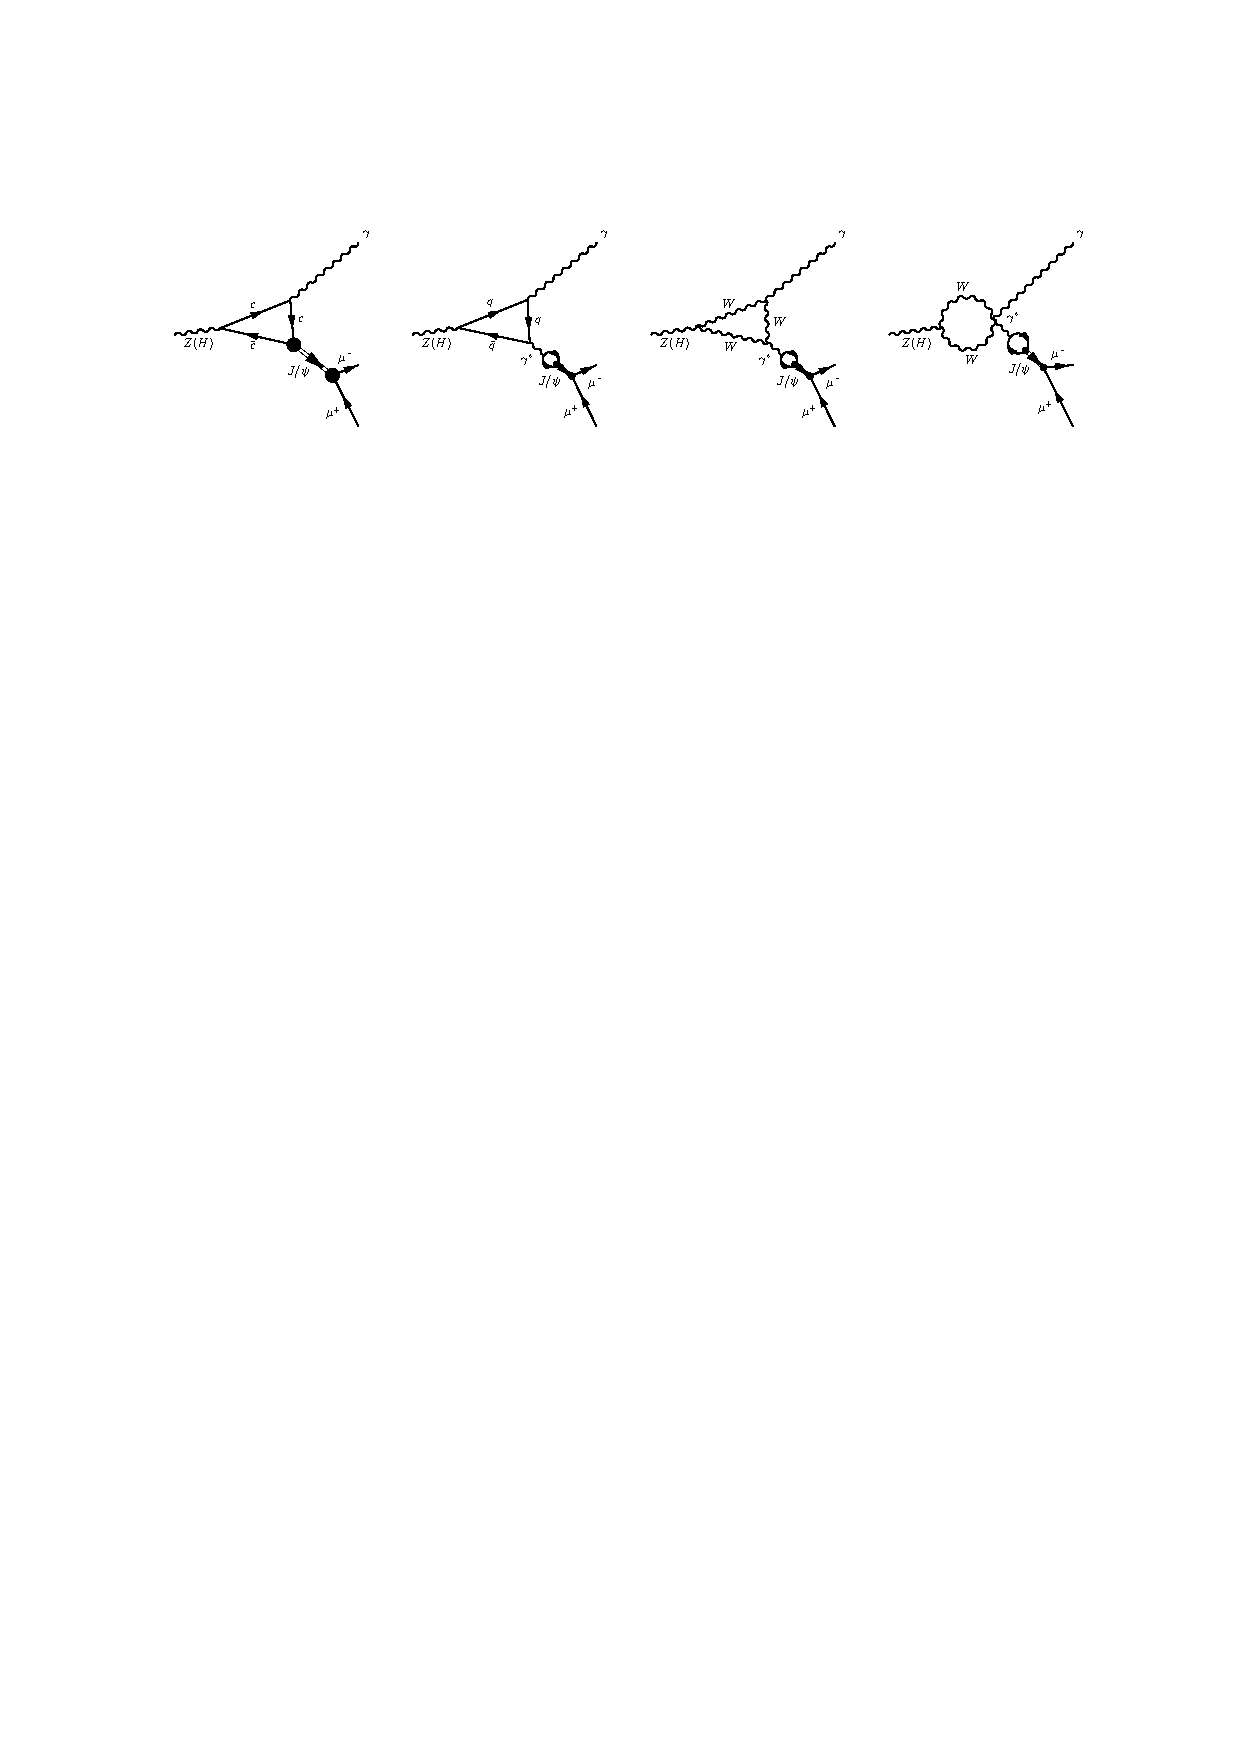
\includegraphics[width=0.9\textwidth]{images/direct_and_indirect_processes.pdf}
			\caption{Lowest order Feynman diagrams for the $\Z$ (or $\H$) $\rightarrow \JPsi\gamma$ decay. The left-most diagram shows the direct and the remaining diagrams the indirect processes\footnotemark.
			\label{im:direct_and_indirect_processes}}
	    \end{figure}
	    \footnotetext{\cite{mainarticle}.}
	    
	    \begin{itemize}
			\item The cumulative yield of the decay is \textcolor{unipd}{proportional to the branching ratio (BR)}.
		\end{itemize}
	\end{frame}
	
	%--------------------------------------------------------------------------
	
	\begin{frame}[t]{\bf Introduction}
        \begin{columns}[c]
            \column{0.5\textwidth}
                \begin{itemize}
                    \item Experimental efforts have only established an \red{upper bound} 200 times the SM predicted value.
                    \item The main challenge is the \red{discrimination} between background and signal $\Rightarrow$ higher luminosity and \red{more efficient trigger} needed.
                \end{itemize}
		
            \column{0.5\textwidth}
                \begin{figure}[c]
                    \centering
                    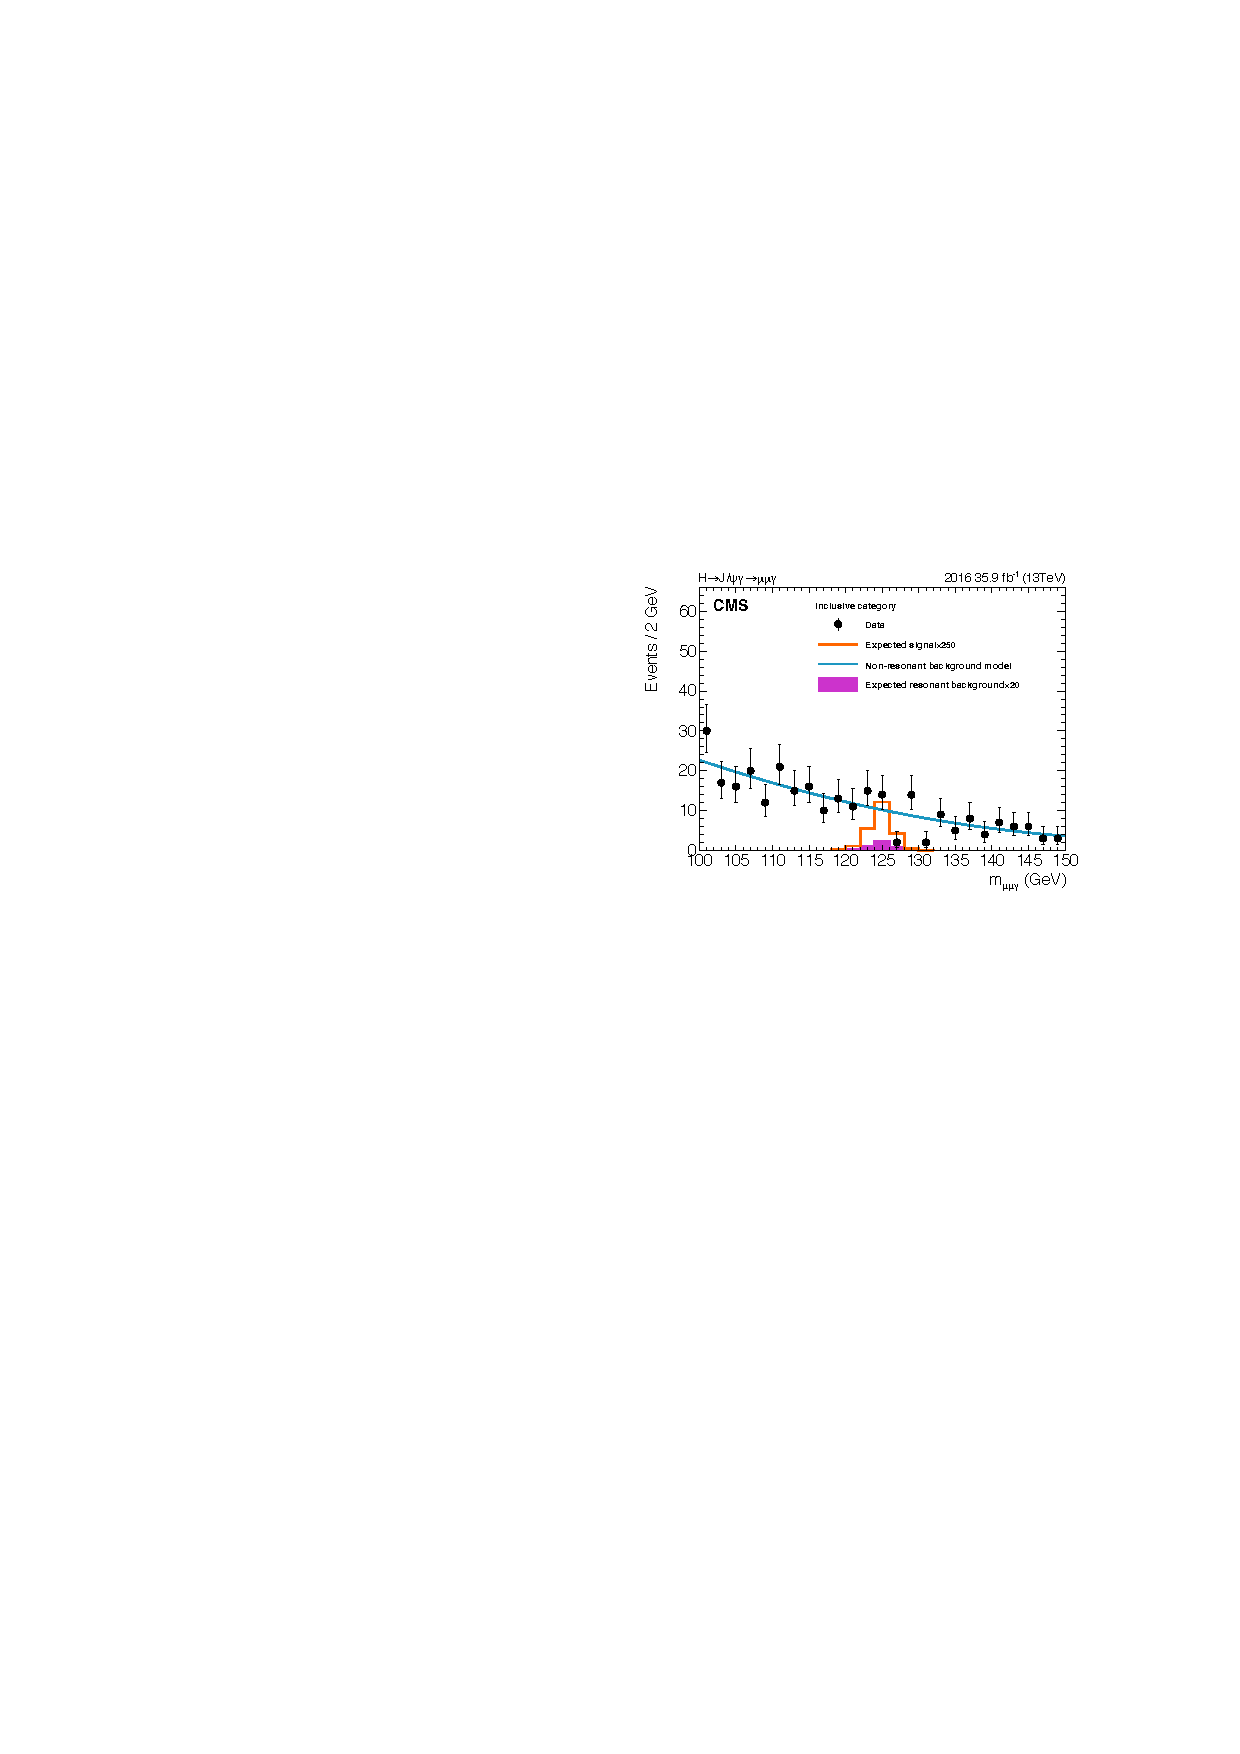
\includegraphics[width=1\textwidth]{images/results-H.pdf}
                    \caption{$m_{\mu\mu\gamma}$ in Higgs boson exotic decay\footnotemark.
                    \label{im:results-H}}
                \end{figure}
	    \end{columns}
	    \footnotetext{\cite{mainarticle}.}
	\end{frame}
	
    %--------------------------------------------------------------------------
	
	\section{Objectives}
        \begin{frame}[t]{\bf Objectives}
            \begin{block}<1->{Trigger}
                In order to filter the amount of data that is recorded from each collision at the LHC, triggers are used. Current High Level Trigger requires the presence of a muon and a photon exceeding 17 and 30 $\GeV$ in the final state.
            \end{block}
            \begin{itemize}
                \item The \red{goal} is then to design a new trigger that can outperform {\it HLT\_Mu17\_Photon30}.
            \end{itemize}
        \end{frame}
	
    %--------------------------------------------------------------------------
	
	\section{Trigger and selection efficiencies}
        \begin{frame}[t]{\bf Trigger and selection efficiencies}
            \vspace{0.3cm}
            \begin{columns}[c]
            \column{0.5\textwidth}
                The \red{trigger efficiency}:
                    \begin{equation*}
                        \red{\varepsilon_{\rm trigger}} = \frac{{\rm \#\ events\ passing\ HLT\ \& \ selection}}{{\rm \#\ events\ passing\ selection}}
                    \end{equation*}
            \column{0.5\textwidth}
                The \red{selection efficiency}:
                \begin{equation*}
                    \red{\varepsilon_{\rm selection}} = \frac{{\rm \#\ events\ passing\ selection}}{{\rm \#\ total\ events}}
                \end{equation*}
            \end{columns}
            \vspace{0.3cm}
            \begin{figure}[c]
                \centering
                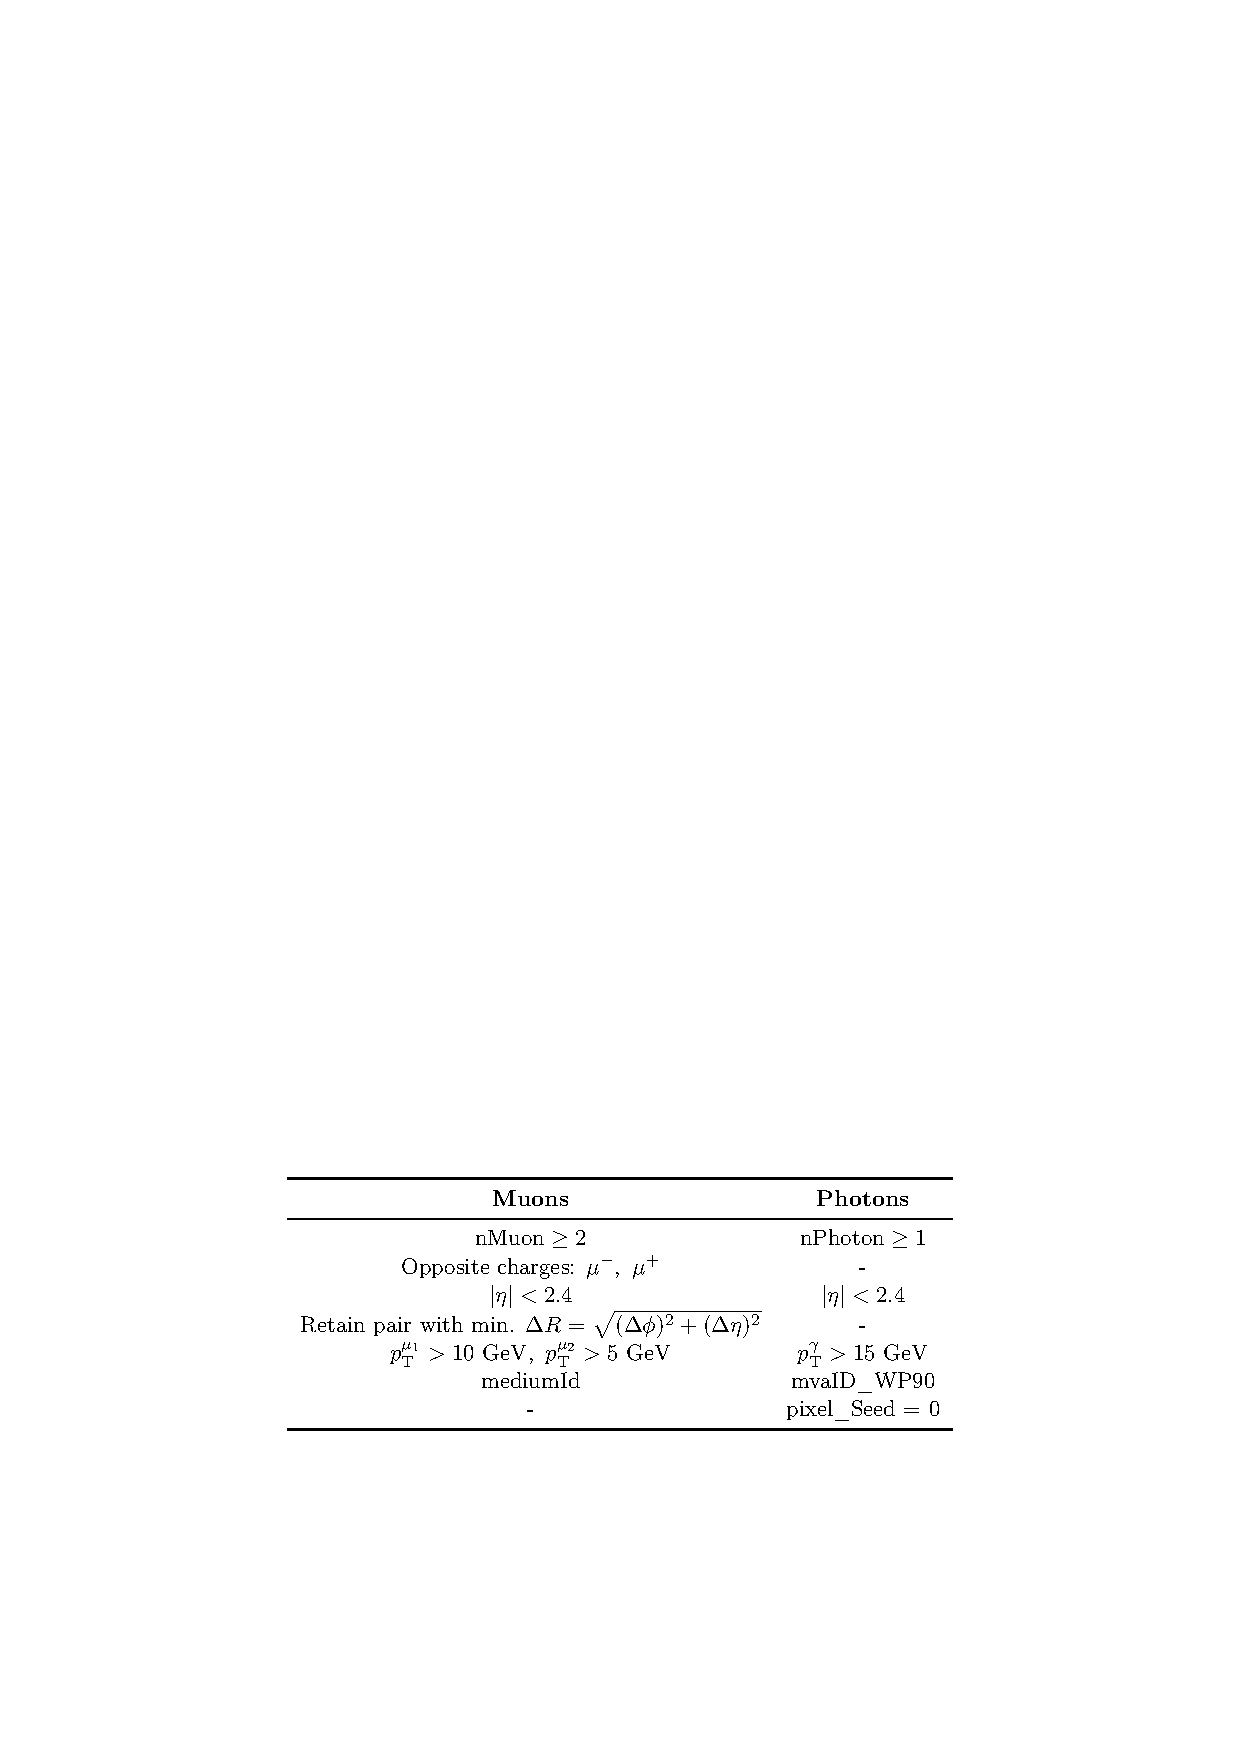
\includegraphics[width=0.6\textwidth]{images/selection_table.pdf}
                \caption{Kinematic, charge and quality selection criteria imposed to the muons and photons in the final state.
                \label{im:selection_table}}
            \end{figure}
        \end{frame}

    %--------------------------------------------------------------------------
	
        \begin{frame}[t]{\bf Example calculation of $\varepsilon$ for {\it HLT\_Mu17\_Photon30}}

        \end{frame}
	
	
	
	
	
	
	
	
	
	
	
	
	
	
	
	
	
	
	
	
	
	
	
	
	
	
	
	
	
    %--------------------------------------------------------------------------
    
	%\begin{frame}[allowframebreaks]{Referencias}
	\begin{frame}{References}
		%\nocite{*}
		\footnotesize{\printbibliography}
		% If too many references, use this command to resize:
	\end{frame}
	
	%--------------------------------------------------------------------------
	
	%\setlength\pdfpagewidth{24.00cm}%
    %\setlength\pdfpageheight{11.00cm}%
	{\usebackgroundtemplate
    {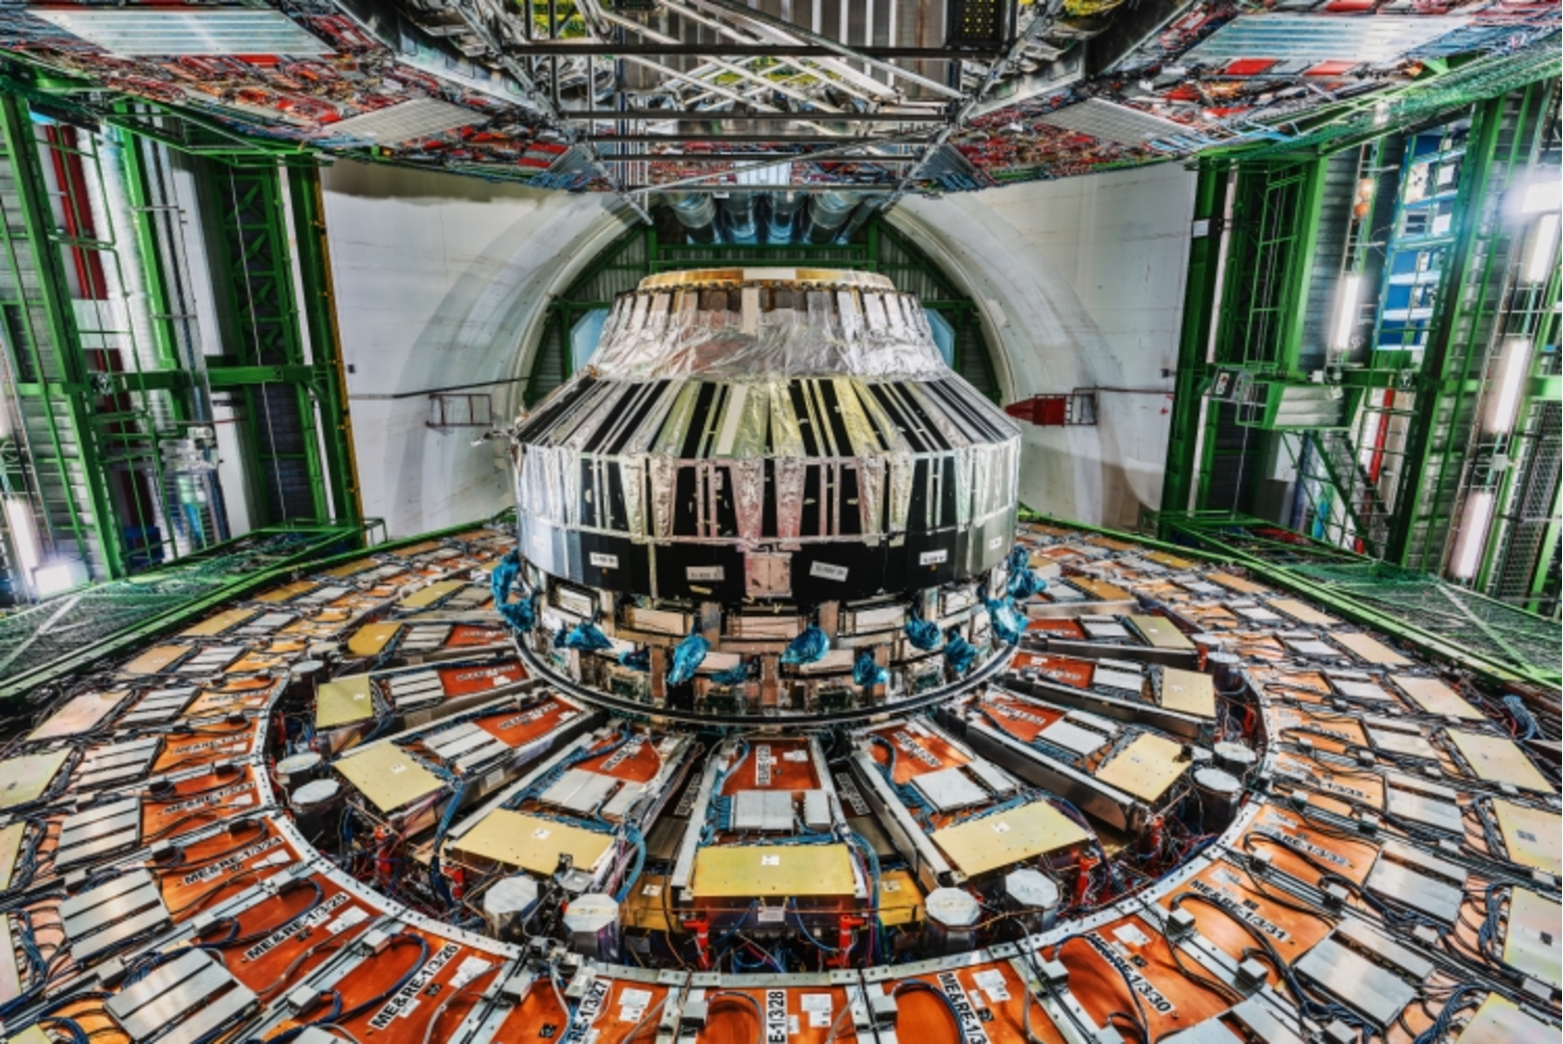
\includegraphics[width=\paperwidth,height=\paperheight]{images/CMS-wallpaper2.pdf}}
	\begin{frame}
    	\thispagestyle{empty}
    	\vspace{-3.cm}
    	\begin{center}
            {\bf\Huge{\textcolor{unipd}{\hl{Thanks for your attention!}}}}
        \end{center}
	\end{frame}}
	
    %--------------------------------------------------------------------------
    
\end{document}